本节给出程序运行结果以及最终恢复得到的明文。实验开始时，先将目标密文拆分为 $IV,C_1,C_2,C_3$ 四个分组，并验证原始密文能够通过服务器的 PKCS\#7 填充检查。服务器返回填充正确，说明 oracle 接口可正常使用，后续攻击可以继续进行。
运行结果如下图:
\begin{figure}[H]
    \centering
    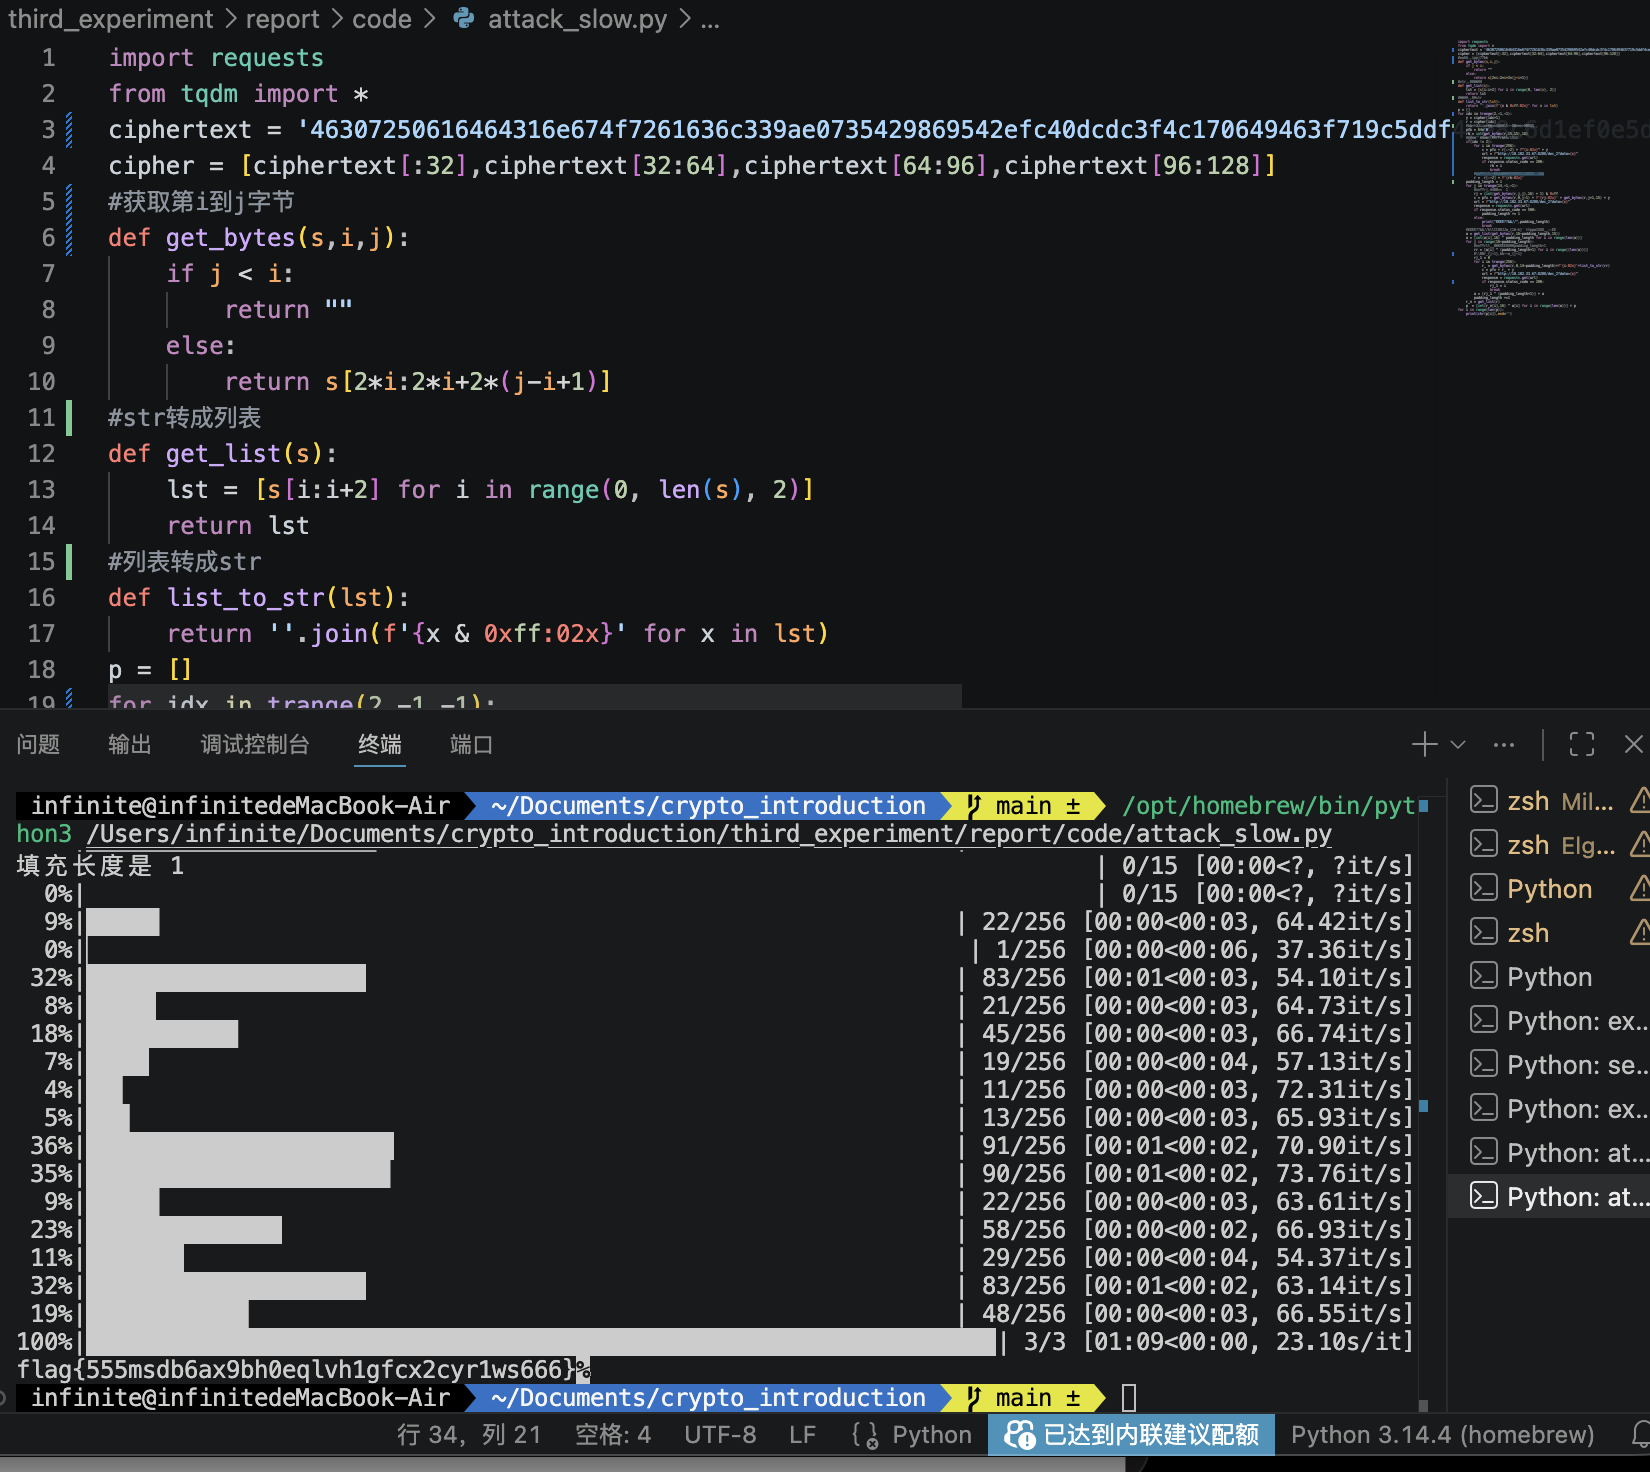
\includegraphics[width = 0.75\textwidth]{figures/attack_1_result.png}
    \caption{代码运行结果}
\end{figure}

\subsection{分组恢复结果}
程序依次对三个目标密文分组进行恢复，最终得到的明文分组结果如表 \ref{tab:plaintext-blocks} 所示。

\begin{table}[H]
    \centering
    \caption{各明文分组恢复结果}
    \label{tab:plaintext-blocks}
    \begin{tabular}{|c|p{7.2cm}|p{4.0cm}|}
        \hline
        分组 & 明文十六进制表示 & ASCII 表示 \\
        \hline
        $P_1$ & \texttt{666c61677b353535 6d73646236617864} & \texttt{flag\{555msdb6axd} \\
        \hline
        $P_2$ & \texttt{3962683065716c76 683167666378326b} & \texttt{9bh0eqlvh1gfcx2k} \\
        \hline
        $P_3$ & \texttt{6379723177733636 367d060606060606} & \texttt{cyr1ws666\}} \\
        \hline
    \end{tabular}
\end{table}
从表中可以看到，第三个明文分组的末尾为 \texttt{06 06 06 06 06 06}。这说明原始明文在最后补入了 6 个 PKCS\#7 填充字节，因此这些字节不属于真实消息内容。

\subsection{完整明文恢复结果}

将三个明文分组顺次拼接后，可以得到带填充的完整明文，其十六进制表示为
\begin{center}
    \ttfamily\small
    666c61677b3535356d73646236617864\\
    3962683065716c76683167666378326b\\
    6379723177733636367d060606060606
\end{center}
去除末尾 6 个字节的 PKCS\#7 填充后，真实明文的十六进制表示为
\begin{center}
    \ttfamily\small
    666c61677b3535356d73646236617864\\
    3962683065716c76683167666378326b\\
    6379723177733636367d
\end{center}
将其按 UTF-8 字符串解码，最终恢复得到 5 号目标密文对应的明文为
\begin{center}
    \fbox{\texttt{flag\{555msdb6axd9bh0eqlvh1gfcx2kcyr1ws666\}}}
\end{center}
这一结果与三个分组的逐块恢复结果是能够相互对应的，也说明程序恢复出的中间状态和最终明文是一致的。
